% !TeX root = ../DistributedConsensus.tex
% !TeX spellcheck = en_GB
\chapter{Validation of Histories}
\label{chap:consensusindcr}
	This chapter defines how histories from malicious events are identified and removed.
	
	\newpar We introduce malicious agents in a given distributed DCR graph. These agents can corrupt data in many ways. Therefore it is desired to have a mechanism which can observe, identify, and handle these corruptions in a predictable way. 
	
	Traditionally malicious agents can tamper with messages in transfer by altering, replaying and withholding messages. We assume that any of these kinds of corruption of messages in transfer are not present in this system. How a system can handle these kinds of corruptions is examined in \todo[inline]{Henvis til en artikel der udforsker disse traditionelle typer "snyd"}.
	
	\newpar Therefore the kinds of cheating examined in this project are the following:
	\begin{definition}
		\textbf{Cheating} is any changing of a history that is not corresponding to what actually happened in the DCR graph.
	\end{definition}
	\todo[inline]{Tilføj rigtig definition.}
	
	\section{Validating histories}
	In order to identify malicious events in a given history, we need to define what a valid history is:
	
		\begin{definition}
			A \textit{\textbf{Valid History}} is a history, for which it applies that all actions happen according to the rules of the DCR graph, abiding serial equivalence and being in a strict partial order. 
		\end{definition}
		
	This also introduces a special kind of cheating:
	
		\begin{definition}
			\textbf{Inconsistent cheating} is the act of manipulating a history in a way where the result is not valid.
		\end{definition}
		
	\subsection{DCR Rules}
	A given execution must abide to the rules of the DCR graph it is part of. That includes the following:
	
	\newpar \textbf{Valid relations}: A given history for an event must only contain actions which represents relations to another event where there exists such a relation in the DCR graph definition and vice versa. 
	
	\newpar \textbf{Complete executions}: A given event, $e1$ must have actions for each of its outgoing relation when executing. Each of the counterparts of these actions must have a corresponding action in their history after $e1$ has executed.
	
	\newpar \textbf{Executions only in Valid States}: The history of an event must only contain executions when the event is executable. That is, the event is included and all of its conditions are either excluded or executed.
	
	\subsection{Serial Equivalence Rules}
	A given execution must abide the rules of serially equivalence. That includes the following:
	
	\newpar \textbf{Non-disrupted Executions}: A given event, $e1$ must not contain ingoing relations or execute starts when already executing. Furthermore if an execution is started, it must also finish. The exception to the rule of ingoing relations is when an event has a relation to itself in which case an incoming action is allowed.
	
	\newpar \textbf{Wait for Complete Execution}: A given event, $e1$ must be affected by all its ingoing relations from an event, $e2$ when $e2$ executes before anything else happens. The exception to the rule is when an event has a relation to itself in which case actions from the execution are allowed before the next incoming action happens. 
	
	\subsection{History Graph Rules / Strict Partial Ordering / Lamport Logical Clocks}
	A given history must abide the rules of being a strict partial order. That includes the following:
	
	\newpar \textbf{Total Order of Local Timestamps}: Every action in the history of an event must be in strict total order according to the timestamp.
	
	\newpar \textbf{Total Order of Counterpart Timestamps}: In the history of an event actions with the same counterpart ID must have its counterpart timestamp in strict total order.  The exception to the rule is when an event has a relation to itself in which case counterpart timestamp can be be lower. \todo{example}
	
	\newpar \textbf{Outgoing Relations Timestamp Order}: When an action is part of an outgoing relation the counterpart's corresponding action's timestamp must be higher than the outgoing one.
	
	\newpar Together, these rules makes sure that no cycles can exist.
    \todo[inline]{Indsæt figurer og algoritmer der kan opdage hver af disse typer snyd.}
    
	\subsection{Simulation}
    \todo[inline]{Simulation bruges til at finde events som har executed uden at være executable. Skriv dette afsnit.}
%	Executions only in Valid States is a special case which is non trivial to check. HOW DO WE DO. ALSO WE DONT KNOW IF IT IS THE EVENT ITSELF DOING BAD BEHAVIOR OR A CONDITION REPLIED WITH LYING DATA.
	
%	\newpar If any of these rules are not adhered to an event must be malicious, since any well functioning event would not be able to such a create history. Thereby allowing us to identify and, if wanted, remove this subset of corruption types.
	
	\section{Consistent Cheating}
	Until now we have examined inconsistent cheating, but malicious events are also able to cheat consistently:
	\begin{definition}
		\textbf{Consistent cheating} is the act of manipulating data in a way where the history is still valid.
	\end{definition}
	
	\newpar Consistent cheating can take a number of forms:

	\newpar \textbf{Non correct timestamps}: A malicious event manipulates the timestamps of the actions in the history, while still maintaining order in both local and counterpart timestamps.
	
	\newpar \textbf{Non correct number of executions}: The history of a malicious event states that it has executed either fewer or more times than it has done, and in doing so might also have outgoing relation actions.
	
	\subsection{Cases}
	Detecting and identifying consistently cheating events is difficult, because it is not possible to look at a single event's history and determine if it is valid or not. We will now examine how the structure of the DCR graph, and the connection between malicious events contribute to the ability to detect and identifying consistent cheating. The type of relation has no influence on the cases and relations are therefore visualised as a simple arrow from event to event.
	
	\newpar \textbf{Case 1 - Single Malicious Event}: In this case (see \ref{fig:consensus:single-malicious}), the event does not share relations with any other event, there is no one to disagree with any timestamps on actions and, in addition, completely oppose to the fact that an execution has happened or not. Therefore in workflows or subworkflows that include such events, it is not possible to identify or even observe if any kind of consistent cheating has happened.
	
	\begin{figure}[H]
		\centering
		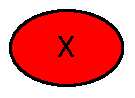
\includegraphics[]{5validation/images/1.pdf}
		\caption{}
		\label{fig:consensus:single-malicious}
	\end{figure}
	
	
	\newpar \textbf{Case 2 - Single Malicious Event With Relation to Self}: This case (see \ref{fig:consensus:single-malicious-with-relation}), just like case 1, in this case there are no one but the event itself to disrupt the cheating and therefore it is not possible to observe or identify consistent cheating.
	
	\begin{figure}[H]
		\centering
		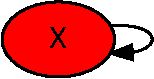
\includegraphics[]{5validation/images/5.pdf}
		\caption{}
		\label{fig:consensus:single-malicious-with-relation}
	\end{figure}
	
	\newpar \textbf{Case 3 - Single Malicious Event With Relation to Good Event}: In this case (see \ref{fig:consensus:single-malicious-with-good-relation}), the malicious event has a relation to a correctly working event. If the malicious event tries to cheat by changing the timestamps, it can do so in two ways. It can try to change the timestamps of the actions corresponding to the relation with the correctly working event, but in that case the two events will not agree on what happened and we are able to observe that one of them must cheat. Due to the fact that any of the two events could be malicious and change the timestamps it would not be possible to identify which of the two are evil.
	If the timestamp changes are on action which not related to the good event then it is not possible to observe nor identify. 
	\todo[inline]{figur eksempler til tekst}
	In the same way when looking at more or fewer executions, the relation action in the executions should have a counterpart but might not have. In the scenario where there are fewer executions the correctly working event will have actions with no counterpart and therefore it is only possible to observe and not identify this kind of cheating. 
	
	\begin{figure}[H]
		\centering
		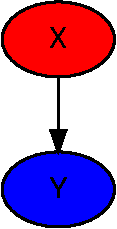
\includegraphics[]{5validation/images/3.pdf}
		\caption{}
		\label{fig:consensus:single-malicious-with-good-relation}
	\end{figure}
	
	\newpar \textbf{Case 4 - Single Good Event With Relation to Single Malicious Event}: In this case (see \ref{fig:consensus:single-good-with-malicious-relation}), a good event has a relation to a malicious event. Similarly to case 3 timestamp changes are observable due to the same factors, but instead of disagreeing on the outgoing relation in this case the malicious event will disagree on whether the good event executed or not. Due to the fact that when the malicious event executes the good event will not have any information about it, because it is not affected by that execution, the malicious event is able change the number of executions to its liking.
	 
	\begin{figure}[H]
		\centering
		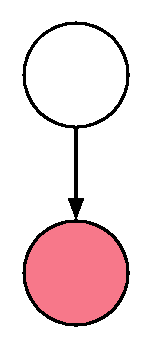
\includegraphics[]{5validation/images/2.pdf}
		\caption{}
		\label{fig:consensus:single-good-with-malicious-relation}
	\end{figure}
	
	\newpar \textbf{Case 5 - Single Good and Single Malicious Event with Relations to each other}: In this case (see \ref{fig:consensus:single-good-with-twoway-malicious-relation}), the situation is similar to that of case 3 and provides the same ability to observe and identify the cheater.
	
	\begin{figure}[H]
		\centering
		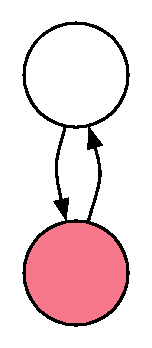
\includegraphics[]{5validation/images/6.pdf}
		\caption{}
		\label{fig:consensus:single-good-with-twoway-malicious-relation}
	\end{figure}
	
	\newpar \textbf{Case 6 - Single Malicious Event A with relation to Single Malicious Event B}: In this case (see \ref{fig:consensus:single-malicious-with-twoway-malicious-relation}), two malicious events work in collaboration to manipulate the data. Because a malicious event is also unpredictable, one of the events could function as a correctly functioning event and create the same depicting scenarios as in case 3 and 4, any absence of manipulation actually corresponds to the event functioning correctly.
	
	If it is assumed that both events work in collaboration to manipulate the history, it is both possible to change timestamps in such a way that it is not observable if they agree on the numbers, or observable if they disagree. Furthermore fewer or more executions is equally easily obscured if they agree that they did or did not happen.
	
	\begin{figure}[H]
		\centering
		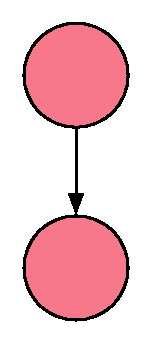
\includegraphics[]{5validation/images/4.pdf}
		\caption{}
		\label{fig:consensus:single-malicious-with-twoway-malicious-relation}
	\end{figure}
	
	\newpar \textbf{Case 7 - Two Malicious Events With Relations To Eachother}: In this case (see \ref{fig:consensus:two-malicious-with-twoway-malicious-relation}), two malicious events work in collaboration with to manipulate data with both their relations. This situation has the same properties as case 6.
	
	\begin{figure}[H]
		\centering
		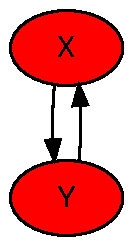
\includegraphics[]{5validation/images/7.pdf}
		\caption{}
		\label{fig:consensus:two-malicious-with-twoway-malicious-relation}
	\end{figure}
	
\todo[inline]{Figurerne ovenfor viser de forskellige situationer. Der skal selvfølgelig knyttes en beskrivelse af situationen, samt i hvilket omfang dette kan opdages til hver figur.}

It becomes apparent that the structure of the DCR graph has a great influence on whether it is possible to observe consistent cheating or not - especially in cases where a lot of malicious events create interconnected or not connected to any other event at all it can be difficult to say anything about the state of the history. One could argue what implications consistent cheating have on subgraphs such as those of case 1 and 2, since their these events have little consequences on the rest of the workflow state and these events can only exist in two states (before and after they are executed) and therefore not being able to handle these kinds of situations is not that big a flaw. The true problems clearly happen in situation 6 and 7 where for example a company can own a sub part of the graph with many events working together to create a falsified image of what has happened. 

